\documentclass[titlepage,landscape]{seminar}
\usepackage{url}
\usepackage{graphicx}
\usepackage{hyperref}
\usepackage{epstopdf}
\usepackage{slides}

\newcommand{\frack}{\frac{1}{k}}

\begin{document}

\myslide{
\heading{Where we're headed}
\[
\Var(P) = \Var(G) + \Var(E)
\]
\vfill
\[
h^2_n = \frac{\Var(A)}{\Var(P)}
\]
\vfill
\[
R = h^2_nS
\]
\vfill So far we've partitioned $V_g$ into $V_a$ and $V_d$ when we
know genotypic values and genotype frequencies, but we still have a
long ways to go.
}

\myslide{
\heading{Genotypic value}
\begin{center}
\resizebox{!}{7cm}{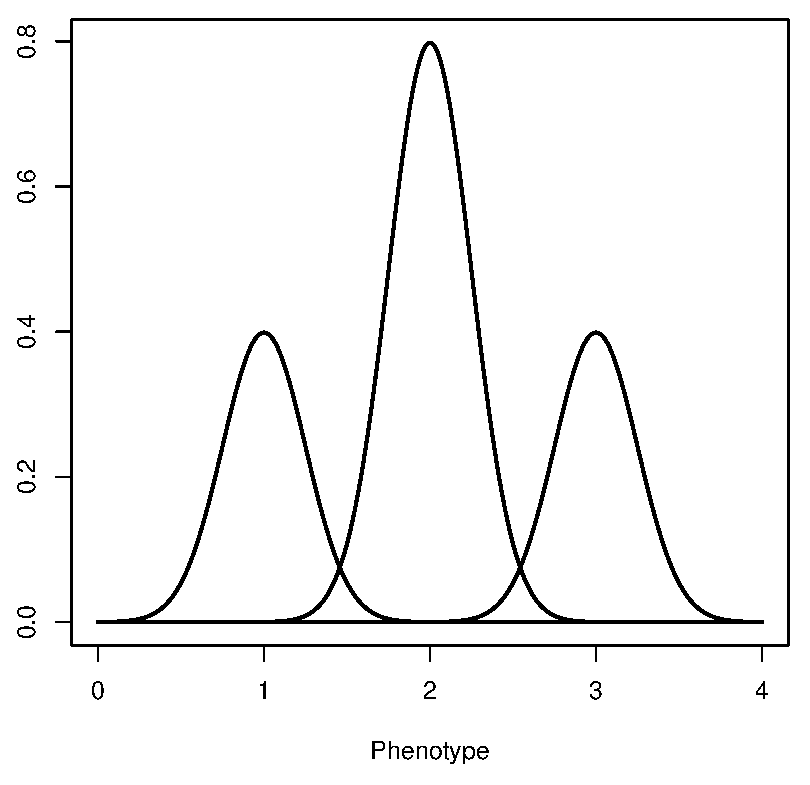
\includegraphics{genotypic-value.eps}}
\end{center}
}

\myslide{
  \heading{Genotypic and additive genotypic values}
\begin{center}
\begin{tabular}{l|ccc}
\hline\hline
Genotype                 & $A_1A_1$    & $A_1A_2$ & $A_2A_2$ \\
\hline
Frequency                & $p^2$       & $2pq$    & $q^2$ \\
Genotypic value          & $x_{11}$    & $x_{12}$ & $x_{22}$ \\
Additive genotypic value & $2\alpha_1$ & $\alpha_1 + \alpha_2$ 
                                                  & $2\alpha_2$ \\
\hline
\end{tabular}
\end{center}
}

\myslide{
  \heading{Partitioning the genetic variance}
\begin{eqnarray*}
V_g &=&\ p^2[x_{11} - {\bar x}]^2 + 2pq[x_{12} - {\bar x}]^2
     + q^2[x_{22} - {\bar x}]^2 \label{eq:v-g} \\
    &=&\ p^2[x_{11} - 2\alpha_1 + 2\alpha_1 - {\bar x}]^2
     + 2pq[x_{12} - (\alpha_1 + \alpha_2) + (\alpha_1 + \alpha_2)
                - {\bar x}]^2 \nonumber \\
     &&\ \ + q^2[x_{22} - 2\alpha_2 + 2\alpha_2 - {\bar x}]^2
     \nonumber \\
    &=&\ p^2[x_{11} - 2\alpha_1]^2 + 2pq[x_{12} - (\alpha_1+\alpha_2)]^2
       + q^2[x_{22} - 2\alpha_2]^2 \nonumber \\
     &&\ + p^2[2\alpha_1 - {\bar x}]^2 + 2pq[(\alpha_1 + \alpha_2) - {\bar x}]^2
       + q^2[2\alpha_2 - {\bar x}]^2 \nonumber \\
     &&\ + p^2[2(x_{11} - 2\alpha_1)(2\alpha_1 - {\bar x})] \\
     &&\ +2pq[2(x_{12} - \{\alpha_1+\alpha_2\})(\{\alpha_1+\alpha_2\} -
     {\bar x})] \nonumber \\
    &&\ +q^2[2(x_{22} - 2\alpha_2)(2\alpha_2 - {\bar x})] \\
    &=& V_a + V_d + 0
\end{eqnarray*}
}

\myslide{
  \heading{Covariance among relatives}

  \begin{center}
\begin{tabular}{ll}
\hline\hline
MZ twins ($\Cov_{MZ}$) & $V_a + V_d$ \\
Parent-offspring ($\Cov_{PO}$)$^1$ & $\left(\frac{1}{2}\right)V_a$ \\
Full sibs ($\Cov_{FS}$) & $\left(\frac{1}{2}\right)V_a +
\left(\frac{1}{4}\right)V_d$ \\
Half sibs ($\Cov_{HS}$) & $\left(\frac{1}{4}\right)V_a$ \\
\hline
\multicolumn{2}{l}{$^1$One parent or mid-parent.}
\end{tabular}
\end{center}
}

\myslide{
  \heading{Evolution of quantitative traits}

  \noindent Linear regression of fitness on phenotype:

\noindent Slope:
\[
\beta_1 = {\Cov(w,x) \over \Var(x)}
\]
Intercept
\[
\beta_0 = \bar w - \beta_1 \bar x \quad .
\]
\vfill
Fitnesses:
\begin{eqnarray*}
w_{ij} &=& \int_{-\infty}^\infty w(x) \mbox{\rm dF}_{ij}(x) \\
       &\approx& \int_{-\infty}^\infty (\beta_0 + \beta_1x) \mbox{\rm dF}_{ij}(x) \\
       &=& \beta_0 + \beta_1x_{ij} \\
\bar w &\approx& \beta_0 + \beta_1\bar x \quad .
\end{eqnarray*}
}

\myslide{
  \heading{Evolution of quantitative traits}

  \begin{eqnarray*}
\int_{-\infty}^\infty x w(x) \mbox{\rm dF}_{ij}(x) - x_{ij}\bar w 
              &=& \bar w \left(
                 \int_{-\infty}^\infty {x w(x) \over \bar w} \mbox{\rm
                 dF}_{ij}(x)
                 - x_{ij}
                 \right) \\
              &=& \bar w (x_{ij}^* - x_{ij})
\end{eqnarray*}
\vfill
\begin{eqnarray*}
\Cov(w,x) &=& p^2\bar w(x_{11}^* - x_{11}) + 2pq\bar w(x_{12}^* - x_{12})
              q^2\bar w(x_{22}^* - x_{22}) \\
&=& \bar w(\bar x^* - \bar x)
\end{eqnarray*}
\vfill
\begin{eqnarray*}
\Delta\bar x &=& V_a \left({\bar w(\bar x^* - \bar x) \over
                               V_p} \over \bar w \right) \cr 
             &=& h^2_N (\bar x^* - \bar x) \cr
\end{eqnarray*}
}

\myslide{
\heading{Fisher's Fundamental Theorem of Natural Selection}
  
\begin{center}
\begin{tabular}{l|ccc}
\hline\hline
Genotype                 & $A_1A_1$ & $A_1A_2$ & $A_2A_2$ \\
\hline
Frequency                & $p^2$    & $2pq$    & $q^2$ \\
Fitness                  & $w_{11}$ & $w_{12}$ & $w_{22}$ \\
Additive fitness value   & $2\alpha_1$ & $\alpha_1 + \alpha_2$ &
$2\alpha_2$ \\
\hline
\end{tabular}
\end{center}
\[
\Delta p = \left({{pq} \over 2{\bar w}}\right)
           \left({{d{\bar w}} \over {dp}}\right) \quad .
\]
\[
{\bar w}' = {\bar w} + \left(\Delta p\right)\left({{d{\bar w}} \over {dp}}\right)
            + \left({{(\Delta p)^2} \over 2}\right)
              \left({{d^2{\bar w}} \over {dp^2}}\right) \quad .
\]
Or, equivalently
\[
\Delta {\bar w} = \left(\Delta p\right)\left({{d{\bar w}} \over {dp}}\right)
            + \left({{(\Delta p)^2} \over 2}\right)
              \left({{d^2{\bar w}} \over {dp^2}}\right) \quad .
\]
}

\myslide{
\heading{Fisher's Fundamental Theorem of Natural Selection}

\begin{eqnarray*}
\frac{d{\bar w}}{dp}
 &=& 2pw_{11} + 2(1-p)w_{12} - 2pw_{12} - 2(1-p)w_{22} \\
 &=& 2[(pw_{11}+qw_{12}) - (pw_{12}+qw_{22})] \\
 &=& 2[(pw_{11}+qw_{12}-{\bar w}/2) - (pw_{12}+qw_{22}-{\bar w}/2)] \\
 &=& 2[\alpha_1 - \alpha_2] \\
 &=& 2\alpha
\end{eqnarray*}
\vfill
\begin{eqnarray*}
\frac{d^2{\bar w}}{dp^2}
 &=& 2w_{11} - 2w_{12} - 2w_{12} + 2w_{22} \\
 &=& 2(w_{11} - 2w_{12} + w_{22}) \\
\end{eqnarray*}
\vfill
\begin{eqnarray*}
\Delta {\bar w}
 &=& \left\{\left({{pq} \over {2{\bar w}}}\right)\left({{d{\bar w}} \over {dp}}\right)
      \right\}
    \left({{d{\bar w}} \over {dp}}\right)
    + {{ \left\{\left({{pq} \over {2{\bar w}}}\right)\left({{d{\bar w}} \over {dp}}\right)
      \right\}^2} \over 2}
    [2(w_{11} - 2w_{12} + w_{22})] \\
 &=& \left\{\left({{pq} \over {2{\bar w}}}\right)\left(2\alpha\right)\right\}\left(2\alpha\right)
    + \left\{\left({{pq} \over {2{\bar w}}}\right)\left(2\alpha\right)\right\}^2
    (w_{11} - 2w_{12} + w_{22}) \\
 &=& {{2pq\alpha^2} \over {\bar w}}
    + {{p^2q^2\alpha^2} \over {{\bar w}^2}}(w_{11} - 2w_{12} + w_{22}) \\
 &=& {V_a \over {\bar w}}
    \left\{1 + {{pq} \over {2{\bar w}}}(w_{11} - 2w_{12} + w_{22})\right\} \\
 &\approx& {V_a \over {\bar w}}
\end{eqnarray*}
}

\myslide{
\heading{Selection on multiple traits}

\noindent Selective differential:
\[
{\bf s} = \bar{\bf z}^* - \bar{\bf z}
\]
\vfill
\noindent $W({\bf z})$ is absolute fitness of individual
with phenotype $\bf z$
\[
\bar W = \int W({\bf z})p({\bf z})d{\bf z} \quad .
\]
\noindent Relative fitness (mean relative fitness $=$ 1)
\[
w({\bf z}) = {W({\bf z}) \over \bar W} \quad .
\]
\vfill
\[
\bar{\bf z}^* = \int {\bf z}w({\bf z})p({\bf z})d{\bf z} \quad .
\]
}

\myslide{
\heading{Selection on multiple traits}

\begin{eqnarray*}
{\bf s} &=& \bar{\bf z}^* - \bar{\bf z} \\
        &=& \int {\bf z}w({\bf z})p({\bf z})d{\bf z} - \bar {\bf z} \\
        &=& E(w,z) - \bar w\bar {\bf z} \\
        &=& \Cov(w,z)
\end{eqnarray*}
}

\myslide{
\heading{Selection on multiple traits}

\[
{\bf P} = {\bf G} + {\bf E} \quad .
\]
\vfill
\begin{eqnarray*}
\bar{\bf x}^* - \bar{\bf x} &=& {\bf GP}^{-1}(\bar{\bf z}^* - \bar{\bf z}) \\
\bar{\bf z}'  - \bar{\bf z} &=& {\bf GP}^{-1}(\bar{\bf z}^* - \bar{\bf z}) \\
\Delta\bar{\bf z} &=& {\bf GP}^{-1}{\bf s}
\end{eqnarray*}
\vfill
\[
{\bf \beta} = {\bf P}^{-1}{\bf s}
\]
\begin{eqnarray*}
s_i &=& \sum_{j=1}^n \beta_jP_{ij} \\
    &=& \beta_1P_{i1} + \cdots + \beta_iP_{ii} + \cdots + \beta_nP_{in}
\end{eqnarray*}
}

\myslide{
\heading{Selection on multiple traits}

\begin{center}
\begin{tabular}{l|cc}
\hline\hline
Character & Mean before selection & standard deviation \\
\hline
head      & 0.880                 & 0.034 \\
thorax    & 2.038                 & 0.049 \\
scutellum & 1.526                 & 0.057 \\
wing      & 2.337                 & 0.043 \\
\hline
\end{tabular}
\vskip 4pt
\begin{tabular}{l|cccc}
\hline\hline
          & head & thorax & scutellum & wing \\
\hline
head      & 1.00 & 0.72   & 0.50      & 0.60 \\
thorax    &      & 1.00   & 0.59      & 0.71 \\
scutellum &      &        & 1.00      & 0.62 \\
wing      &      &        &           & 1.00 \\
\hline
\end{tabular}
\end{center}
}

\myslide{
\heading{Selection on multiple traits}

\begin{center}
\begin{tabular}{l|cccc}
\hline\hline
Character & $s$    & $s'$  & $\beta$ & $\beta'$ \\
\hline
head      & -0.004 & -0.11 & -0.7 $\pm$ 4.9 & -0.03 $\pm$ 0.17 \\
thorax    & -0.003 & -0.06 & 11.6 $\pm$ 3.9$^{**}$ & 0.58 $\pm$ 0.19$^{**}$
\\
scutellum & -0.16$^*$ & -0.28$^*$ & -2.8 $\pm$ 2.7 & -0.17 $\pm$ 0.15 \\
wing      & -0.019$^{**}$ & -0.43$^{**}$ & -16.6 $\pm$ 4.0$^{**}$ & -0.74 $\pm$
0.18$^{**}$ \\
\hline
\end{tabular}
\end{center}
}

\myslide{
  \heading{Association mapping}

  \noindent Na\"ive approach. Regression of phenotype on genotype:
  \[
    y_i = x_{ij}\beta_j + \epsilon_{ij} \quad ,
  \]
  where $y_i$ is the phenotype of individual $i$, $x_{ij}$ is the
  genotype of individual $i$ at locus $j$ (0, 1, 2), and
  $\epsilon_{ij} \sim \mbox{N}(0, \sigma^2)$ is the error.
  \vfill
  {\color{red}\bf PROBLEM}: Individuals may be similar to one another
  because of genetic similarity not reflected in the particular
  markers chosen, e.g., relatedness within a population, population
  structure
}

\myslide{
  \heading{Association mapping}

  \noindent Better approach. Regression of phenotype on genotype with
  a random effect reflecting genetic similarity at markers not
  included in the analysis

  \[
    y_i^{(k)} = x_{ij}\beta_j + \phi^{(k)} + \epsilon_{ij}
  \]

  In general $\phi^{(k)}$ may reflect a general measure of
  relatedness, usually estimated from SNPs.
}

\myslide{
\heading{Warfarin resistance}
\vfill
\begin{center}
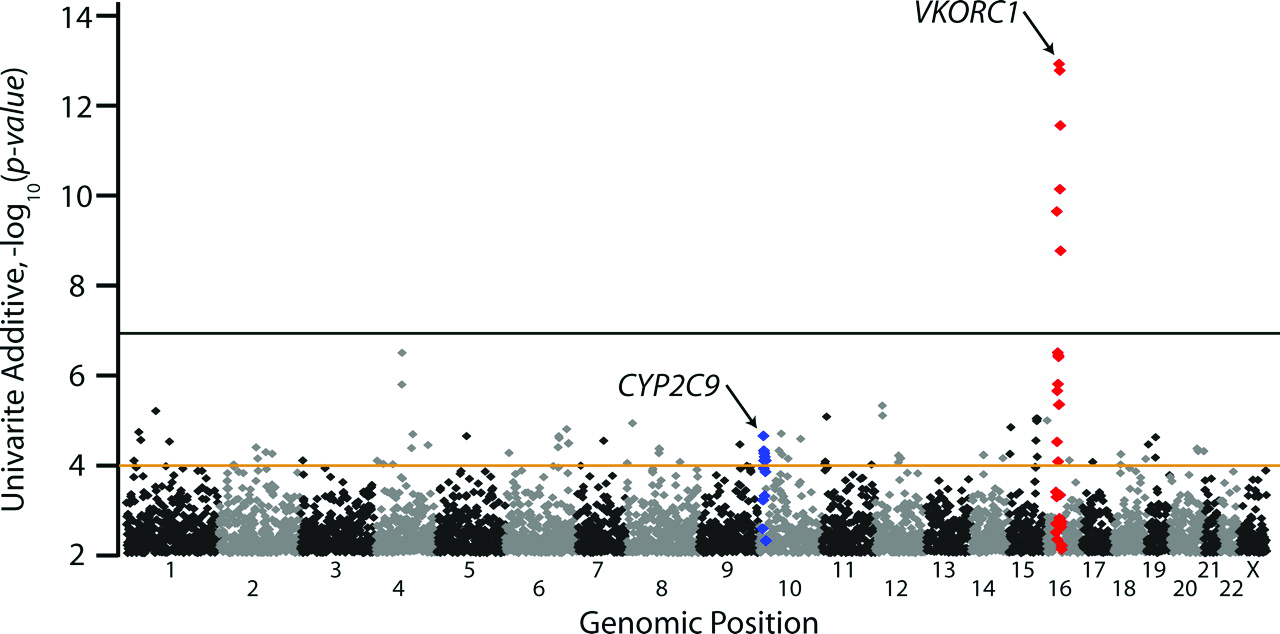
\includegraphics[width=0.9\textwidth]{GWAS-warfarin.eps}
\end{center}
}

\myslide{
  \heading{Warfarin resistance}

  \vfill
\begin{center}
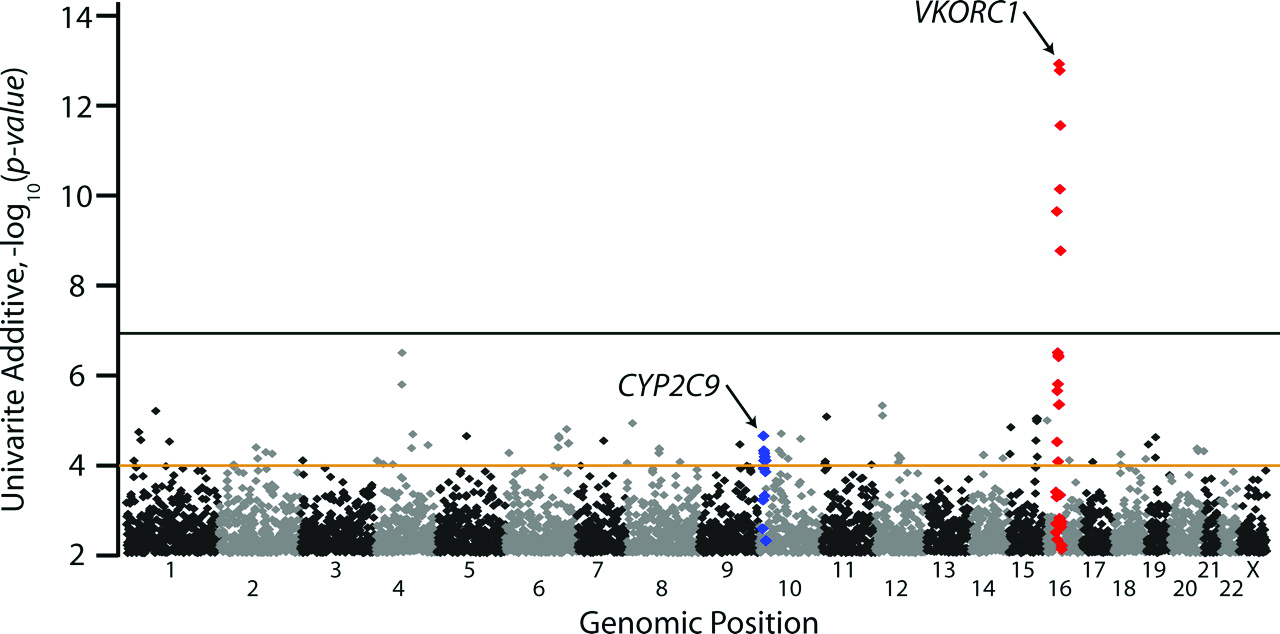
\includegraphics[width=0.9\textwidth]{GWAS-warfarin.eps}
\end{center}
\vfill
25\% of variance in dose associated with {\it VVKORC1}
}

\myslide{
  \heading{Significance vs. effect size}

  At least 400 loci associated with differences in height in
  humans. How much effect can any one locus have?
}

\myslide{
  \heading{Significance vs. effect size}

  \begin{center}
    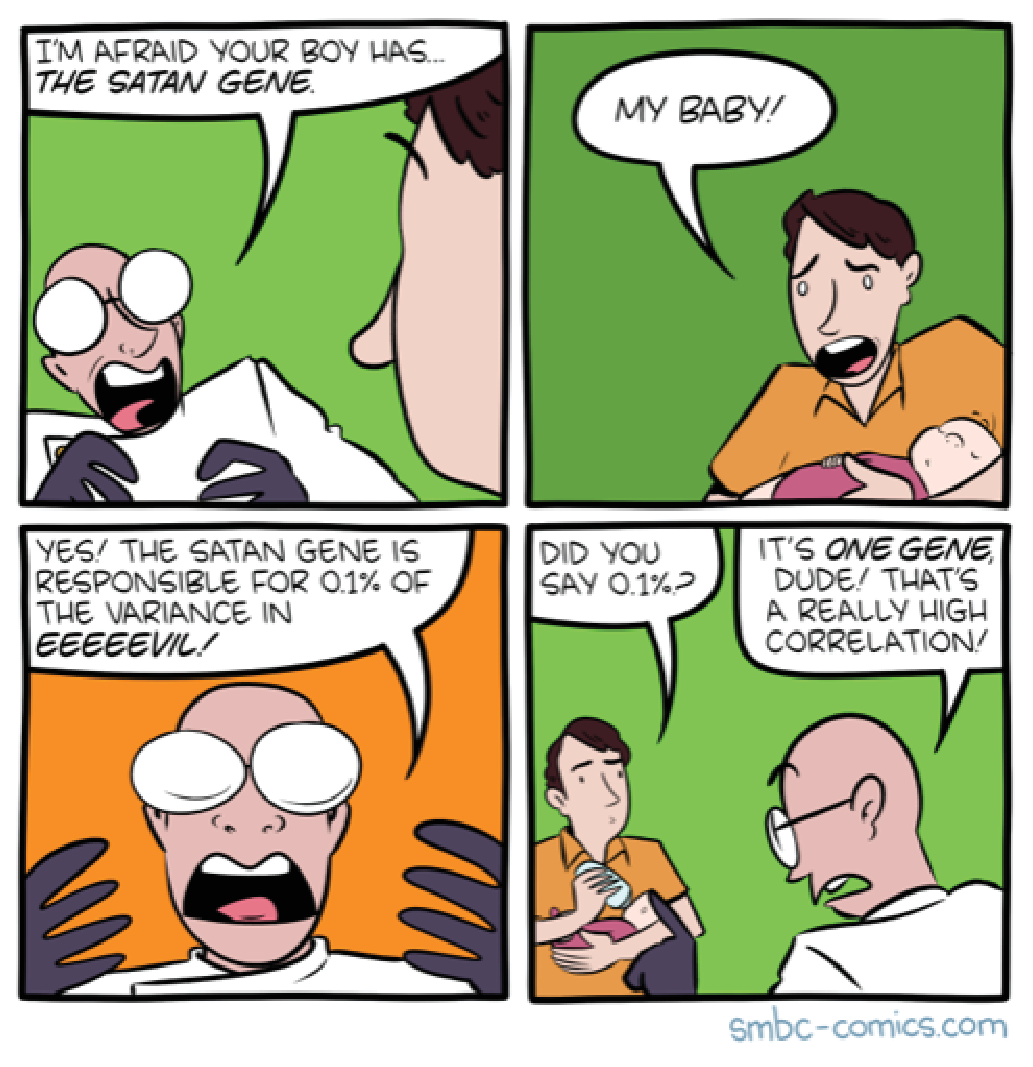
\includegraphics[height = 0.9\textheight]{GWAS-small-effect.eps}
  \end{center}
}

\myslide{
  \heading{Two-locus population genetics}
\begin{center}
\begin{tabular}{lcccc}
Gamete    & $A_1B_1$ & $A_1B_2$ & $A_2B_1$ & $A_2B_2$ \\
Frequency & $x_{11}$ & $x_{12}$ & $x_{21}$ & $x_{22}$
\end{tabular}
\end{center}
\vfill
If alleles are arranged randomly into gametes then,
\begin{eqnarray*}
x_{11} &=& p_1p_2 \\
x_{12} &=& p_1q_2 \\
x_{21} &=& q_1p_2 \\
x_{22} &=& q_1q_2 \quad ,
\end{eqnarray*}
where $p_1 = \hbox{freq}(A_1)$ and $p_2 = \hbox{freq}(A_2)$.
}

\myslide{
  \heading{Two-locus population genetics}

  In general,
  \begin{eqnarray*}
    x_{11} &=& p_1p_2 + D \\
    x_{12} &=& p_1q_2 - D \\
    x_{21} &=& q_1p_2 - D \\
    x_{22} &=& q_1q_2 + D \\
    \\
    D &=& x_{11}x_{22} - x_{12}x_{21}
  \end{eqnarray*}

  \vfil
  
  $D$: gametic disequilibrium

  \vfill
}

\myslide{
  \heading{Two-locus population genetics}
\[
\begin{array}{ccccccc}
    &\mu_1            &     &      &     &\mu_2 \\
A_1 &\rightleftharpoons& A_2 &\qquad& B_1 &\rightleftharpoons& B_2
\quad , \\
    &\nu_1            &     &      &     &\nu_2 
\end{array}
\]
\vfill
\begin{eqnarray*}
\frac{\mbox{E}(D^2)}{\mbox{E}(p_1(1-p_1)p_2(1-p_2))}
&\approx& \frac{1}{3 + 4N_er}
\end{eqnarray*}
}

\myslide{
  \heading{Two-locus population genetics}
\begin{center}
\begin{tabular}{c|cccc|cc|c}
\hline\hline
           & \multicolumn{4}{c|}{Gamete frequencies} 
           & \multicolumn{2}{c|}{Allele frequencies} \\
Population & $A_1B_1$ & $A_1B_2$ & $A_2B_1$ & $A_2B_2$ 
           & $p_{i1}$ & $p_{i2}$ & $D$ \\
\hline
1          & 0.24     & 0.36     & 0.16    & 0.24
           & 0.60     & 0.40     & 0.00 \\
2          & 0.14     & 0.56     & 0.06    & 0.24
           & 0.70     & 0.20     & 0.00 \\
Combined   & 0.19     & 0.46     & 0.11    & 0.24
           & 0.65     & 0.30     & -0.005 \\
\hline
\end{tabular}
\end{center}
}

\myslide{
  \heading{Two-locus population genetics}

  Remember that
  \[
    x_{11} = p_1p_2  + D
  \]
  \vfill
\begin{eqnarray*}
D_i &=& x_{11,i} - p_{1i}p_{2i} \\
D_t &=& \bar x_{11} - \bar p_1\bar p_2 \\
\bar x_{11} &=& \frac{1}{K} \sum_{k=1}^K x_{11,k} \\
\bar p_1 &=& \frac{1}{K} \sum_{k=1}^K p_{1k} \\
\bar p_2 &=& \frac{1}{K}\sum_{k=1}^K p_{2k}
\end{eqnarray*}
}

\myslide{
  \heading{Two-locus population genetics}
\begin{eqnarray*}
D_t &=& \bar x_{11} - \bar p_1\bar p_2 \\
    &=& \frac{1}{K} \sum_{k=1}^K x_{11,k} - \bar p_1\bar p_2 \\
    &=& \frac{1}{K} \sum_{k=1}^K (p_{1k}p_{2k} + D_k) - \bar p_1\bar p_2 \\
    &=& \frac{1}{K} \sum_{k=1}^K (p_{1k}p_{2k} - \bar p_1\bar p_2) + \bar D \\
    &=& \mbox{Cov}(p_1, p_2) + \bar D \quad ,
\end{eqnarray*}
}

\myslide{
  \heading{Two-locus population genetics}
\begin{eqnarray*}
\mbox{Cov}(p_1, p_2) &=& 0.5(0.6-0.65)(0.4-0.3) + 0.5(0.7-0.65)(0.2-0.3) \\
                     &=& -0.005 \\
\bar x_{11}          &=& (0.65)(0.30) - 0.005 \\
                     &=& 0.19 \\
\bar x_{12}          &=& (0.65)(0.7) + 0.005 \\
                     &=& 0.46 \\
\bar x_{21}          &=& (0.35)(0.30) + 0.005 \\
                     &=& 0.11 \\
\bar x_{22}          &=& (0.35)(0.70) - 0.005 \\
                     &=& 0.24 \quad .
\end{eqnarray*}
}

\myslide{
  \heading{Association mapping}

  \noindent Better approach. Regression of phenotype on genotype with
  a random effect reflecting genetic similarity estimated from genetic
  markers 

  \[
    y_i^{(k)} = x_{ij}\beta_j + \phi^{(k)} + \epsilon_{ij}
  \]

  In general $\phi^{(k)}$ may reflect a general measure of
  relatedness, usually estimated from SNPs.

  But even with a measure of relatedness the association between a
  locus and a phenotype might still reflect population structure, not
  a causal relationship.
}

\myslide{
  \heading{Genomic prediction}

  \noindent Instead of a locus-by-locus analysis, predict phenotype
  using a multiple regression.

  \[
    y_i^{(k)} = \sum_j x_{ij}\beta_j + \phi^{(k)} + \epsilon_{ij}
  \]

  \noindent Use $\sum_j x_{ij}\beta_j$ as a {\it polygenic score}.

  Note: The same caveat about causal interpretation applies here as
  with causal interpretation of a measure of association.
}

\myslide{
  \heading{Natural selection on height in humans}

  \noindent Allele frequency estimates from

  \begin{itemize}

  \item Myocardial Infarction Genetics consortium (MIGen)

  \item Population Reference Sample (POPRES)

  \end{itemize}

  \noindent Compare allele frequencies at loci associated with height
  in two samples (MIGEN)

  \begin{itemize}
  
  \item 247 US individuals of northern European ancestry

  \item 254 Spanish individuals

  \item Compare magnitude of allele frequency difference with 10,000
    randomly selected SNPs with similar mean allele frequencies.

  \end{itemize}

}

\myslide{
  \heading{Natural selection on height in humans}

  \noindent Results

  \begin{itemize}

    \item Alleles associated with increased height were significantly
      more frequent in the ``northern'' population than in the
      ``southern'' population

    \item Similar results from the same kind of analysis with POPRES
      data 

  \end{itemize}

  \noindent CAUTION: These associations could be spurious if ancestry
  was not fully accounted for.

}

\myslide{
  \heading{Natural selection on height in humans}

  \noindent GWAS in Genetic Investigation of ANthropometric
  Traits~(GIANT)

  \begin{itemize}

  \item Careful control of ancestry in GWAS
    
  \item ``Control'' SNPs associated with increased height in GIANT
    more frequent in ``northern'' population

  \item Magnitude of allele frequency differences at 1400 SNPs most
    strongly associated with height more consistent with a model
    including drift {\it and\/} selection than one including drift
    alone. 

  \end{itemize}
}

\myslide{
  \heading{Natural selection on height in humans}

  \noindent Attempt to replicate findings using samples from UK
  Biobank

  \begin{itemize}

    \item ca. 500,000 individuals in database scored for a variety of
      phenotypes and genotypes at a large number of loci.

    \item Analysed six different data sets including GIANT, four
      subsets of the UK Biobank, and a large sib database

    \item GWAS in each data set identifying 1700 independently
      inherited SNPs

      \item Combined these scores to estimate a polygenic score for
        European and Eurasian populations in the 1000 Genomes and
        Human Origins databases

  \end{itemize}
}

\myslide{
  \heading{Natural selection on height in humans}

  \begin{center}
    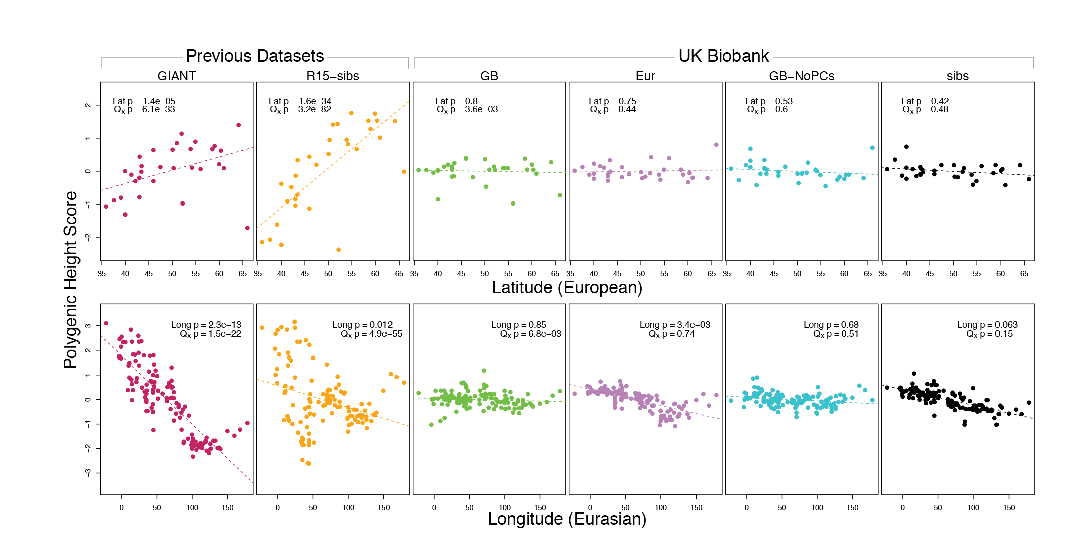
\includegraphics[width=\textwidth]{UK-biobank.eps}
  \end{center}
  
}

\myslide{
  \heading{Natural selection on height in humans}

  \noindent All data sets show real associations with height

  \noindent GIANT and R-15 fail to fully remove confounding variation
  along major geographic axes

  \noindent ``[W]hat once appeared an ironclad example of population
  genetic evidence for polygenic adaptation now lacks any strong
  support.''

}

\myslide{
  \heading{Extrapolating genomic predictions}

  \noindent Stabilizing selection for the same optimum phenotype in
  two genetically isolated populations

  \noindent Expectations

  \begin{itemize}

    \item Same selection: Same phenotypes

    \item Genetic isolation:

      \begin{itemize}

        \item No selection: Populations diverge
        
        \item With selection: \color{red}{\bf ?}

      \end{itemize}

    \end{itemize}

}

\myslide{
  \heading{Extrapolating genomic predictions}

  \begin{center}
    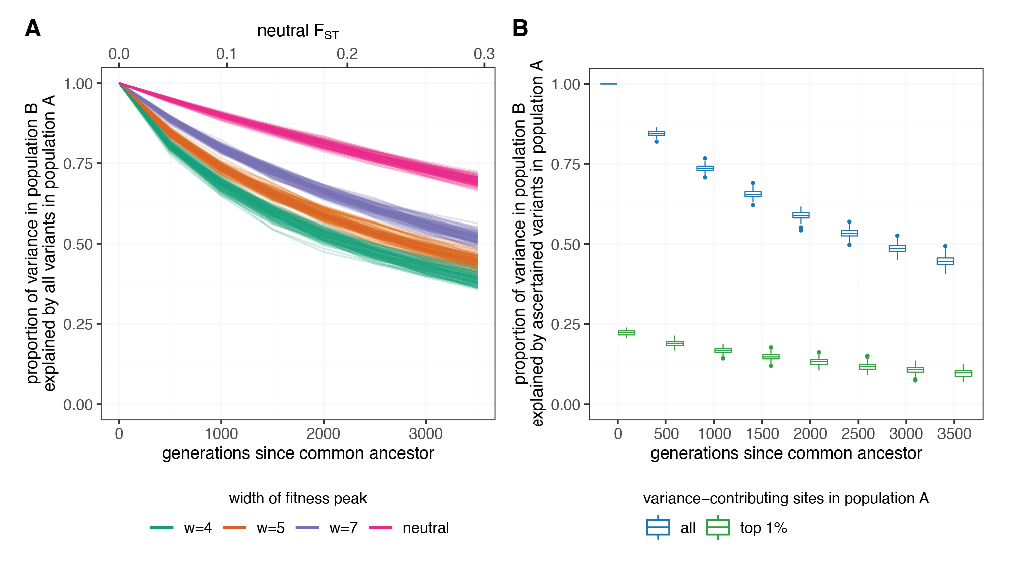
\includegraphics[width=\textwidth]{yair-coop-predictions.eps}
  \end{center}
  
}

\myslide{
  \heading{Genetic redundancy}

  \begin{center}
    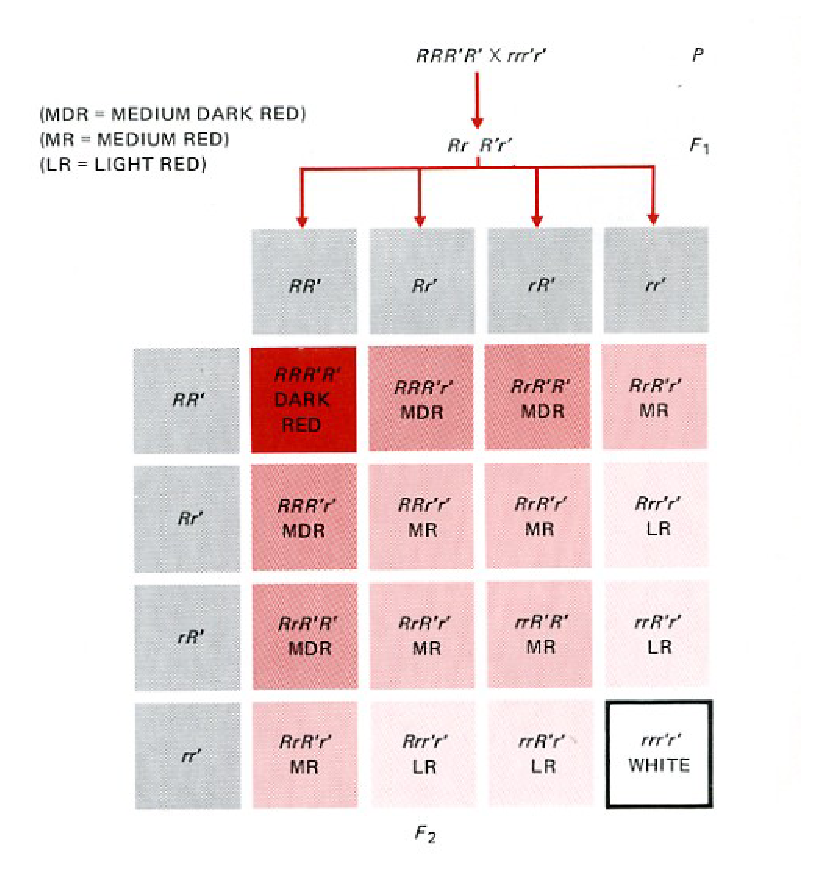
\includegraphics[width=0.6\textwidth]{Nilsson-Ehle.eps}
  \end{center}
  
}

\myslide{
  \heading{Genetic redundancy: isolation by distance}

  \begin{center}
    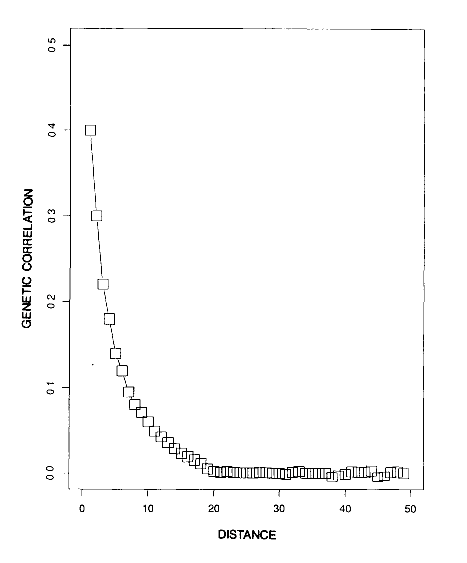
\includegraphics[height=0.8\textheight]{isolation-by-distance.eps}
  \end{center}
  
}

\myslide{
  \heading{Genetic redundancy: isolation by distance}

  \begin{itemize}

  \item Uniform selection for an intermediate genotype

  \item Many genotypes produce the same phenotype

  \item Individuals separated by a long distance evolve independently,
    even though selection produces the same phenotype

  \item Different genotypes produce the same phenotype in different
    parts of the population

  \item Genomic scores estimated in one part of the population won't
    extrapolate to a different part of the population

  \end{itemize}
}

\end{document}
